%%%% Various options for document class.
%%\documentclass[usenatbib, a4paper, 11pt]{aastex}
%%\documentclass[preprint, 11pt, a4paper]{aastex}
%%\documentclass[twocolum]{revtex4}
%%\documentclass{report}
\documentclass[useAMS,usenatbib,onecolumn]{mn2e2}

%\usepackage{psfig,morefloats,url}
%use preprint2 for 2 columns paper.

%% declare any packages used
\usepackage{graphicx}
\usepackage{natbib}
\usepackage{graphicx}
\usepackage{color}
\usepackage{pdfpages}
\usepackage{appendix}
\usepackage{subfigure}
%\usepackage{epsfig}
%\usepackage[dvips]{color}
%\usepackage{aabib}


%\marginparwidth = 25pt
\citestyle{aa}
\addtolength{\topmargin}{-.5in}
%\addtolength{\bottommargin}{-1in}
%% This command added as margins are wrong in mn2e, it appears. 
%% Not needed for other classes




%%%%%%%%%%%%%%%%%%%%%%%%%%%%%%%%%%%%%%

\begin{document}
%% define bibstyle and other definitions
\bibliographystyle{aabib}
%% renew commands
\renewcommand{\labelitemi}{$-$}
\def\la{Ly-$\alpha$ }
\def\py{\textsc{Python} }
\def\tar{\textsc{Tardis} }
\def\cld{\textsc{Cloudy} }
\def\civ{C~\textsc{iv} }
\def\araa{ARAA}
\def\nat{Nature}
\def\apjl{ApJ Letters}
\def\aapr{AAPR}
\def\ssr{SSR}
\def\apj{ApJ}
\def\pasp{PASP}
\def\aap{A\&A}
\def\mnras{MNRAS}
\def\aj{AJ}
\def\rmxaa{RMXAA}

%%%%%%%%%%%%%%%%%%%%%%%%%%%%%%%%%%%%%%
%
%          TITLE AND AUTHORS
%
%%%%%%%%%%%%%%%%%%%%%%%%%%%%%%%%%%%%%%%

\title{Accretion Disk Winds Across The Mass Scale: PhD Transfer Report}


% [Matthews, J.]
\author{James Matthews }
%\\
%Supervisor: Prof. Christian Knigge\\
%{\sl School of Physics \& Astronomy, University of Southampton,
%  Southampton, SO17 1BJ, UK}}


%%%%%%%%%%%%%%%%%%%%%%%%%%%%%%%%%%%%%%
%
%          ABSTRACT
%
%%%%%%%%%%%%%%%%%%%%%%%%%%%%%%%%%%%%%%%

\maketitle


\begin{abstract} 
Broad Absorption Lines (BALs) in the Ultraviolet 
are seen in $\sim20\%$ of Quasi-Stellar Objects (QSOs), and 
are also prominent in spectra of Cataclysmic Variables (CVs)
and some X-ray Binaries. Blue-shifted BALs are the most direct evidence of 
accretion disk `winds' in such systems; mass loaded outflows
emanating from the disk, which may be driven by line forces or
magnetic processes. Here I present an eighteen-month transfer report
on a PhD project that involves using a Monte Carlo radiative transfer code
capable of modeling a variety of systems. The aim is to both
help inform our understanding of the profound connection between 
accretion and mass loss processes, and test unification models in QSOs, CVs and X-ray binaries. 
The code produces synthetic spectra for different viewing angles in
a biconical disk wind model by passing photons through a wind geometry
with a self-consistently computed temperature and ionization structure.
In addition to presenting some relevant background and results so far,
I give an outline of projects and timescales for the remaining work
that will contribute to the final thesis.
\end{abstract}

%\begin{keywords}
%AGN: outflows
%\end{keywords}



%%%%%%%%%%%%%%%%%%%%%%%%%%%%%%%%%%%%%%
%
%          INTRODUCTION
%
%%%%%%%%%%%%%%%%%%%%%%%%%%%%%%%%%%%%%%%
\section{Introduction}
Outflows are crucial to our understanding of accreting systems and are close to ubiquitous 
across approximately 10 orders of magnitude in mass. These outflows can take the form of 
highly collimated radio jets \citep{bellonijet2010}, but can also manifest in 
more mass-loaded `winds' emanating from the accretion disk. The most spectacular evidence of
disk winds is blue-shifted broad absorption in spectral lines, a phenonomenon observed in 
Active Galactic Nuclei (AGN) and Quasi-Stellar Objects (QSOs; Turner \& Miller 2009, 
Weymann et al. 1991\nocite{turnermiller2009, weymann1991}), Cataclysmic Variables 
(CVs; Cordova \& Mason 1982\nocite{cordova1982}) and X-ray Binaries \citep{ioannau2003}.

It is therefore clear that outflows present a unique opportunity to probe the 
proposed {\sl universality} (e.g. Mchardy 2006) of the accretion process across the mass scale, whilst also 
providing potential {\sl unification} models for (see e.g. Elvis 2000\nocite{elvis2000}) each class of object. 
Despite this, the full effect of a disk wind on the observational appearance of an accreting system
remains unclear, and even the fundamental theoretical questions relating to the origin and driving mechanism
for mass loss are unsolved (see Proga 2000 and Proga 2010 for two theoretical reviews). 
These problems affect a variety of astrophysical phenonena. 
Disk winds provide a possible source of AGN feedback, which is a crucial component in galaxy formation and evolution models (e.g. Silk \& Rees 1998\nocite{silkrees1998}).
Cataclysmic variables are one possible progenitor for Type Ia Supernovae, standardisable candles
used to predict the accelerating expansion of the universe, and so the role of accretion in the evolution
of these systems must be understood. Clearly, answering the questions relating to the theory and observational 
imprint of accretion disks and their winds is of wide-ranging significance.


Our team has recently embarked on a project in which a state of the art radiative transfer code, previously
used to model resonance lines in CVs, has been enhanced and improved to be able to model a wider variety of astrophysical
objects and emission mechanisms. The aim of the project is to answer the questions identified above, and to try and understand the
full extent to which the disk wind acts as a spectral `filter' in AGN/QSOs, CVs and X-ray Binaries.
The near ubiquity of outflowing material in accreting systems also implies a deep connection
between accretion and mass loss, so a natural focal point of our work is to assess
the true extent to which accretion disks follow the so-called `$\alpha$-disk' treatment
outlined by \cite{shakurasunyaev1973}. 
Here I present an eighteen-month transfer report for a PhD project. In section 2 I briefly describe the code, 
and some of the methods we employ. In section 3 I provide a description of work carried out so far, and in section 4 I provide a 
plan of remaining work including a thesis outline. Finally, I conclude in section 5.






%%%%%%%%%%%%%%%%%%%%%%%%%%%%%%%%%%%%%%
%
%          RAD TRANSFER THEORY
%
%%%%%%%%%%%%%%%%%%%%%%%%%%%%%%%%%%%%%%%
\section{Method and Approach}

\py is a Monte Carlo radiative transfer code which uses the Sobolev approximation.  
It expands on the work of SV93 and also incorporates techniques described by
Lucy (1999a, 1999b, 2002, 2003). The code is first described by \cite{LK02},
who synthesized the UV spectra of CVs, successfully reproducing P-Cygni resonance line profiles
whilst solving self-consistently for the thermal balance and ionization structure in the wind
according to the method of \cite{LM93}. \py has since been used with application
to QSO wind modeling \citep{higginbottom2013}, which involved a new ionization scheme to deal with the
more complex power-law spectrum, and encorporation os processes such as Compton scattering in order
to correctly treat X-ray radiation transfer. In addition, \cite{simmacro2005} modeled
Brackett and Pfund line profiles in YSOs using \py, which involved
implementing a `macro-atom' line transfer mode.


\subsection{Macro-atoms}

Previously, \py used a two-level atom approximation \cite[see e.g.][]{mihalas} for its treatment of lines. This approximation works well when treating so-called `resonance lines' (such as \civ, O\textsc{vi}), 
in which the excited electron is strongly coupled to the ground state, but when a level is primarily populated from above then this becomes a poor representation. To reproduce recombination lines, it is therefore
important to use an improved line transfer technique and level population solver.

By quantising matter into `macro-atoms', and radiant and kinetic energy into energy packets, 
Lucy (2002, 2003\nocite{lucy2002, lucy2003}; hereafter L02, L03) showed that it is possible 
to asymptotically reproduce the emisssivity of a gas in statistical equilibrium 
without simplifying the treatment of line transfer. A full description of the scheme 
is well beyond the scope of this report (consult L02, L03), but the `take-home' message is
that the macro-atom scheme allows a full treatment of recombination cascades,
with all possible transition paths available to an excited electron.
While Sim et al. (2005) applied this technique to
a Hydrogen-only model, we are now able to adopt a hybrid scheme. Hydrogen and Helium both produce
prominent recombination lines in optical spectra of CVs (see section 3), and so it is important
to be able to treat them as full
macro-atoms. The other species in our model are treated as so-called `simple-ions'; They still
follow the indivisible packet constraint but are simplified to two level atoms
as in LK02. This allows one to preserve the fast treatment of resonance lines by 
produce an improved representation of recombination, which is import for both the 
lines and also the recombination {\sl continuum} which may potentially be responsible for filling in the
Balmer jump.



\subsection{Code Validation}

Python has previously been tested against a number of radiative transfer and
photoionization codes. Comparisons of ionization balance with \cld \citep{cloudy2013} 
can be found in LK02 and H13 showing excellent agreement, we have also conducted comparisons
of ionization and spectral synthesis with the Supernova code \tar. \tar is described by
\citep{kerzendorfsim} and the spectral comparisons can be found therein.

In addition to these code validation efforts, I have also conducted tests of
the macro atom scheme in \py to verify that it does indeed solve for level populations correctly
and produces the correct level emissivities. The left panel of figure~\ref{seaton} shows a comparison
between our level emissivities for the Balmer series compared with analystic calculations
by \cite{seaton1959}, showing good agreement in both the Case A and Case B limits 
(see Osterbrock (1989) for a discussion of these two commonly used approximations).
The right panel of figure~\ref{seaton} shows a comparison of Helium I level populations (the most
complex ion we currently treat as a macro-atom) between \py and \tar models. Considering the 
two codes use different atomic data and \tar currently has a complete treatment of
collisions between radiatively forbidden transitions, the factor of $<2$ agreement is 
encouraging 

\begin{figure}
\mbox{
\subfigure{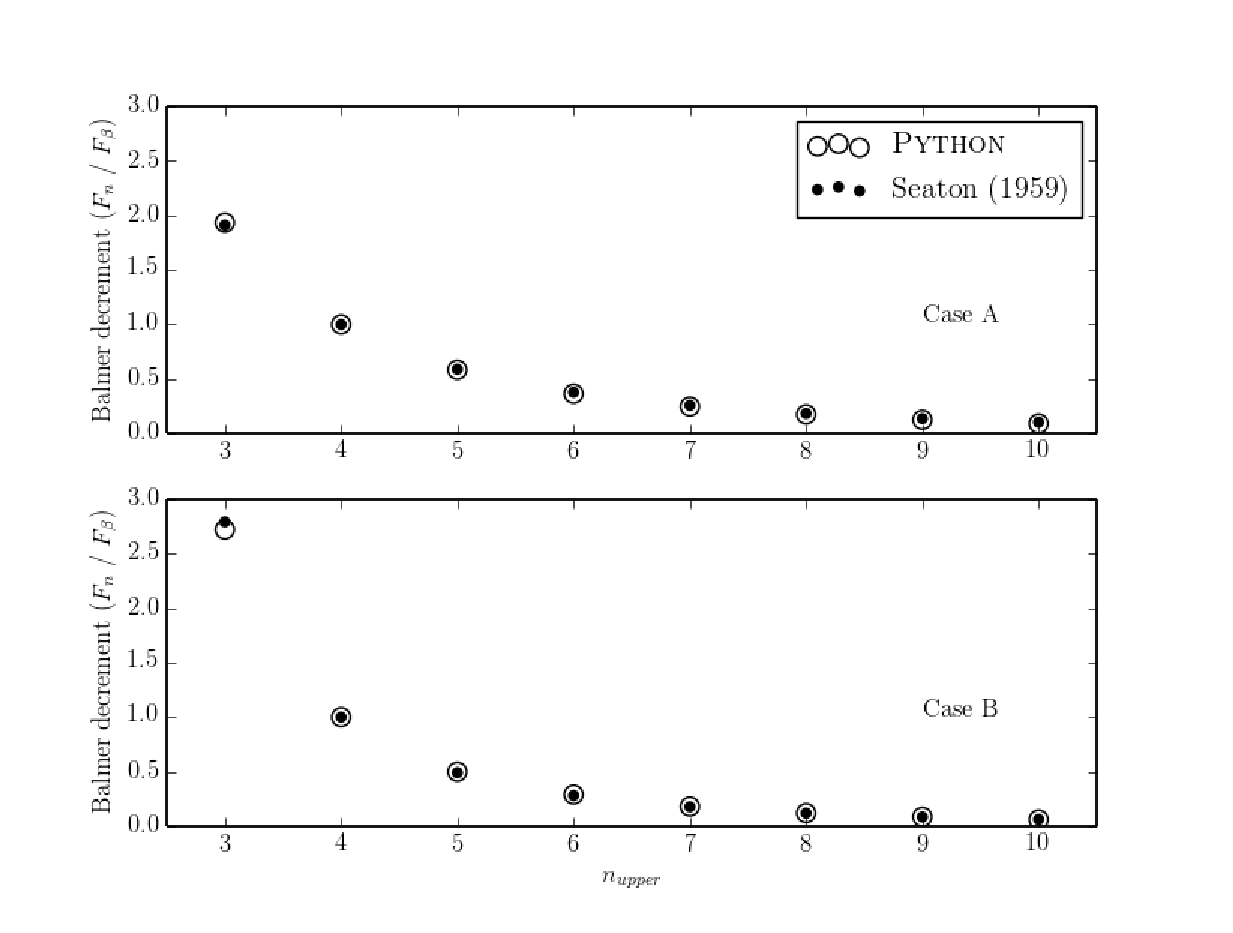
\includegraphics[width=0.45\textwidth]{figures/seaton_emissiv.eps}} 
\quad
\subfigure{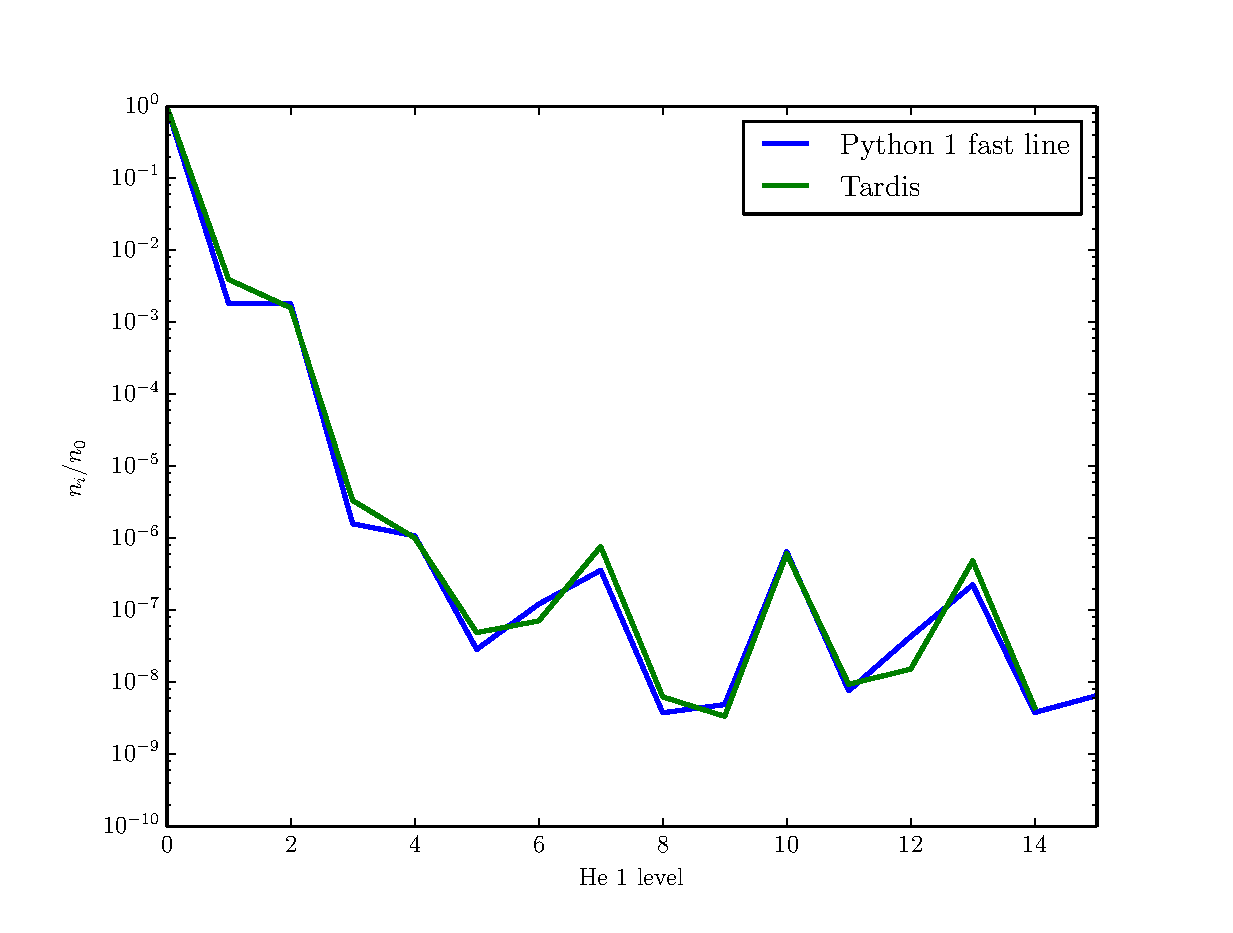
\includegraphics[width=0.45\textwidth]{figures/hepops.eps}}  
}
\caption{
Left: Balmer decrements (level emissivities as a fraction of the $H\beta$ $4\rightarrow2$ transition)
for a Hydrogen only model in the case A and case B limits. Large open circles show
the test model in \py, and filled circles show Seaton's predictions.
Right: Level populations of an example cell with bound-free processes
to excited levels disabled compared to a \tar calculation with the same physical conditions. 
The cell in question has $n_e = 10^8$~cm$^{-3}$, $T_e = 30,000$~K, $T_R = 40,000$~K
and a dilution factor of $W=???$. We also adopt $\tau_{sobolev} = 0$ 
(optically thin limit).
}
\label{seaton}
\end{figure}

% \begin{figure}
% \centering
% 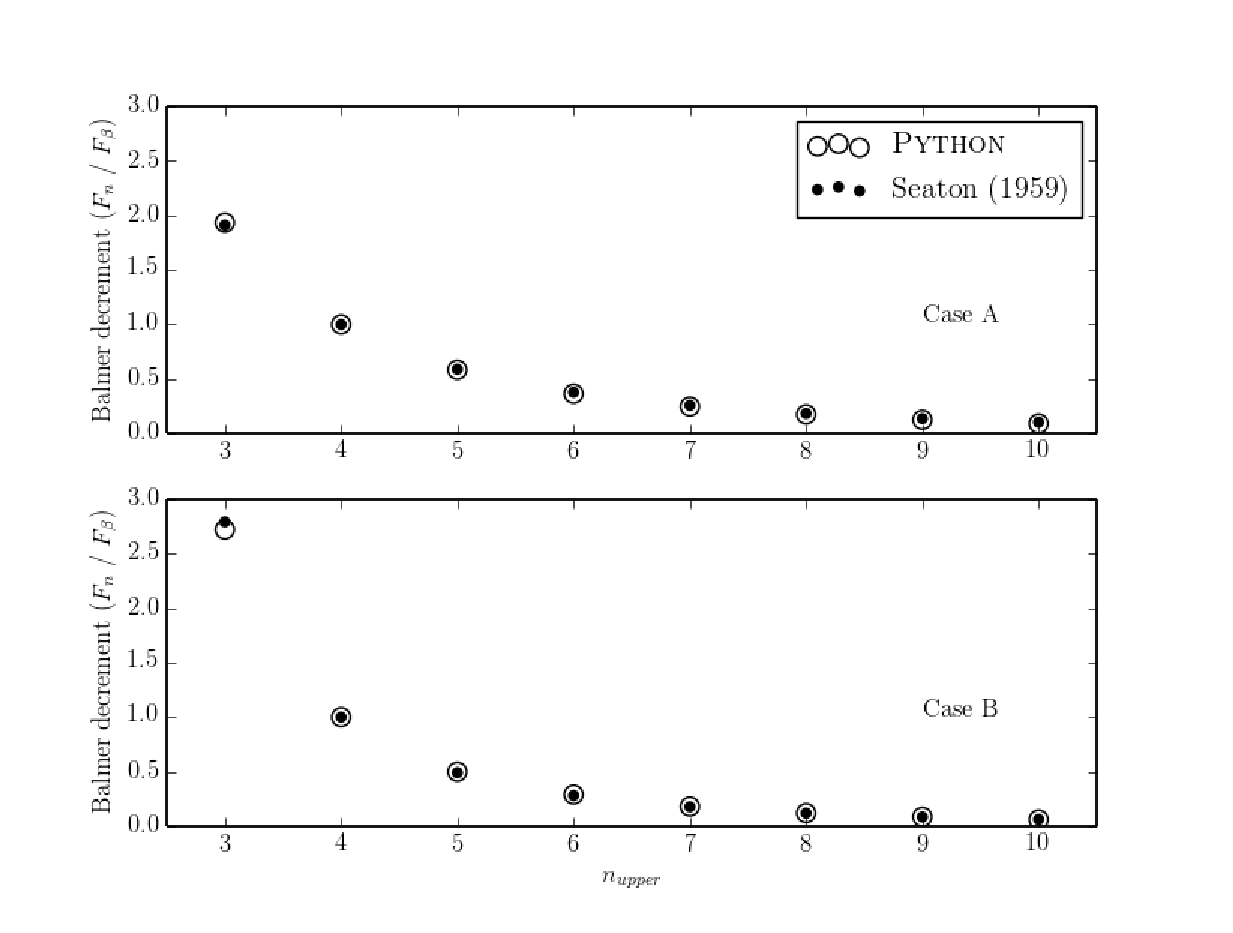
\includegraphics[width=0.6\textwidth]{figures/seaton_emissiv.eps}
% \caption{
% Balmer decrements (level emissivities as a fraction of the $H\beta$ $4\rightarrow2$ transition)
% for a Hydrogen only model in the case A and case B limits. Large open circles show
% the test model in \py, and filled circles show Seaton's predictions.
% }
% \label{seaton}
% \end{figure}


% \begin{figure}
% \centering
% 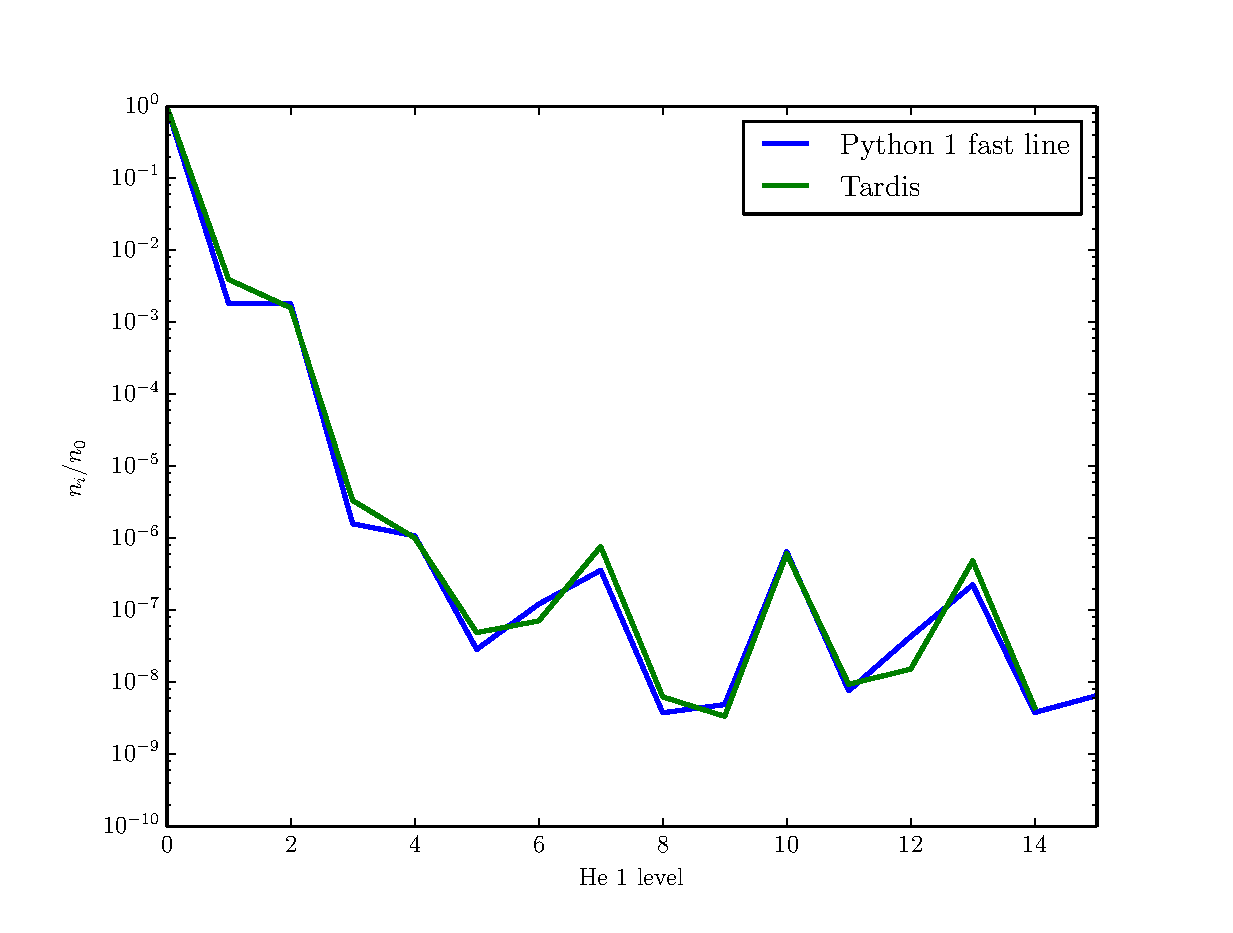
\includegraphics[width=0.6\textwidth]{figures/hepops.eps}
% \caption{Level populations of an example cell with bound-free processes
% to excited levels disabled compared to the calculation carried out with \tar. 
% The cell in question has $n_e = 10^8$~cm$^{-3}$, $T_e = 30,000$~K, $T_R = 40,000$~K
% and a dilution factor of $W=???$. We also adopt $\tau_{sobolev} = 0$ 
% (optically thin limit).}
% \label{hepops}
% \end{figure}

%%%%%%%%%%%%%%%%%%%%%%%%%%%%%%%%%%%%%%%


%%%%%%%%%%%%%%%%%%%%%%%%%%%%%%%%%%%%%%
%
%         RESULTS
%
%%%%%%%%%%%%%%%%%%%%%%%%%%%%%%%%%%%%%%%


\section{The Disk Wind Contribution to the Optical Spectra of Cataclysmic Variables}

Cataclysmic variables (CVs) are systems in which a white dwarf accretes matter from a donor
star via Roche-lobe overflow. In non-magnetic, disk-dominated systems this accretion
is mediated by an accretion disk which forms around the white dwarf. 
Nova-like (NL) variables are a particular subclass of object in which the accretion disk
is in a permanent state of relatively high accretion rate 
($\dot{M} \sim 10^{-8}$~M$_{\odot}$~yr$^{-1}$), making them the perfect laboratories to 
test the $\alpha$-disk model.

For over three decades, it has been known that winds emanating from the accretion disk
are important in shaping the ultraviolet spectra of high-state CVs (Heap 1978), 
the most spectacular evidence being the P-Cygni like profiles of resonance lines such as 
C${\textsc {iv}}$ (see e.g. Cordova \& Mason 1982\nocite{cordova1982}).

While the effect of the wind on the UV is at least partially clear, it may also have more subtle 
effects across the spectral range. It has been proposed that an accretion disk wind
can cause single-peaked emission line profiles in the optical \citep{MC96}, 
such as those seen in Nova-like variables and SW Sex stars \citep{HSK86, DR95}.
It is particularly telling that single-peaked lines can be seen even in eclipse, suggesting 
that a spatially extensive wind may be the source of emission.
%%(Honeycutt, Schlegel, \& Kaitchuck 1986; Dhillon \& Rutten 1995). 
In addition, \cite{KLWB98} suggested
that recombination continuum emission from a disk wind or atmosphere
could be responsible for filling in the Balmer absorption edge, explaining 
the absence of a pronounced `Balmer jump' in optical spectra of CVs.

\subsection{A Biconical Wind CV Model}

We follow LK02 in adopting a biconical wind geometry originally outlined by Schlosman \& Vitello (1993; SV93\nocite{SV93}).
This geometry is shown in figure~\ref{cartoon}. 
A smooth, biconical disk wind rises from the accretion disk between radii $r_{min}$ and $r_{max}$. 
The covering fraction of the wind is controlled by the opening angles of the wind, $\theta_{min}$ and 
$\theta_{max}$. As in LK02, we follow SV93's power law velocity profile. 

\begin{figure}
\centering
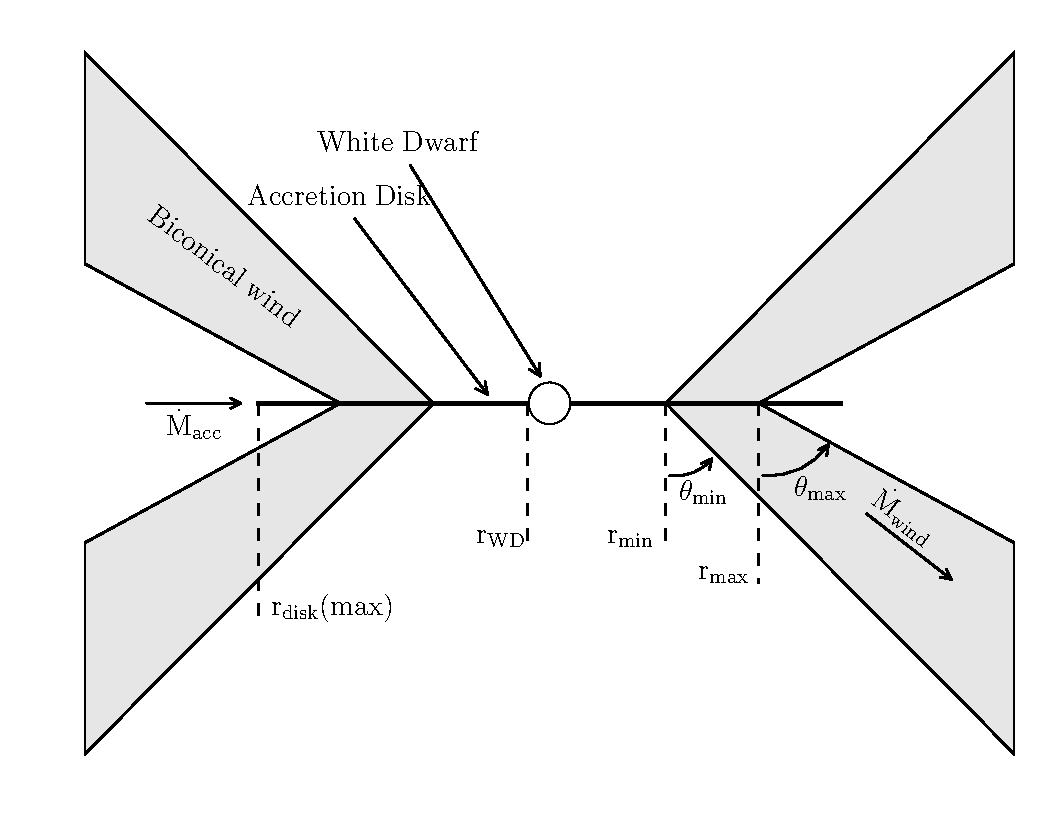
\includegraphics[width=0.5\textwidth]{figures/fig1.eps}
\caption{Cartoon illustrating the geometry and kinematic properties of the CV wind model.}
\label{cartoon}
\end{figure}

\begin{figure}
\centering
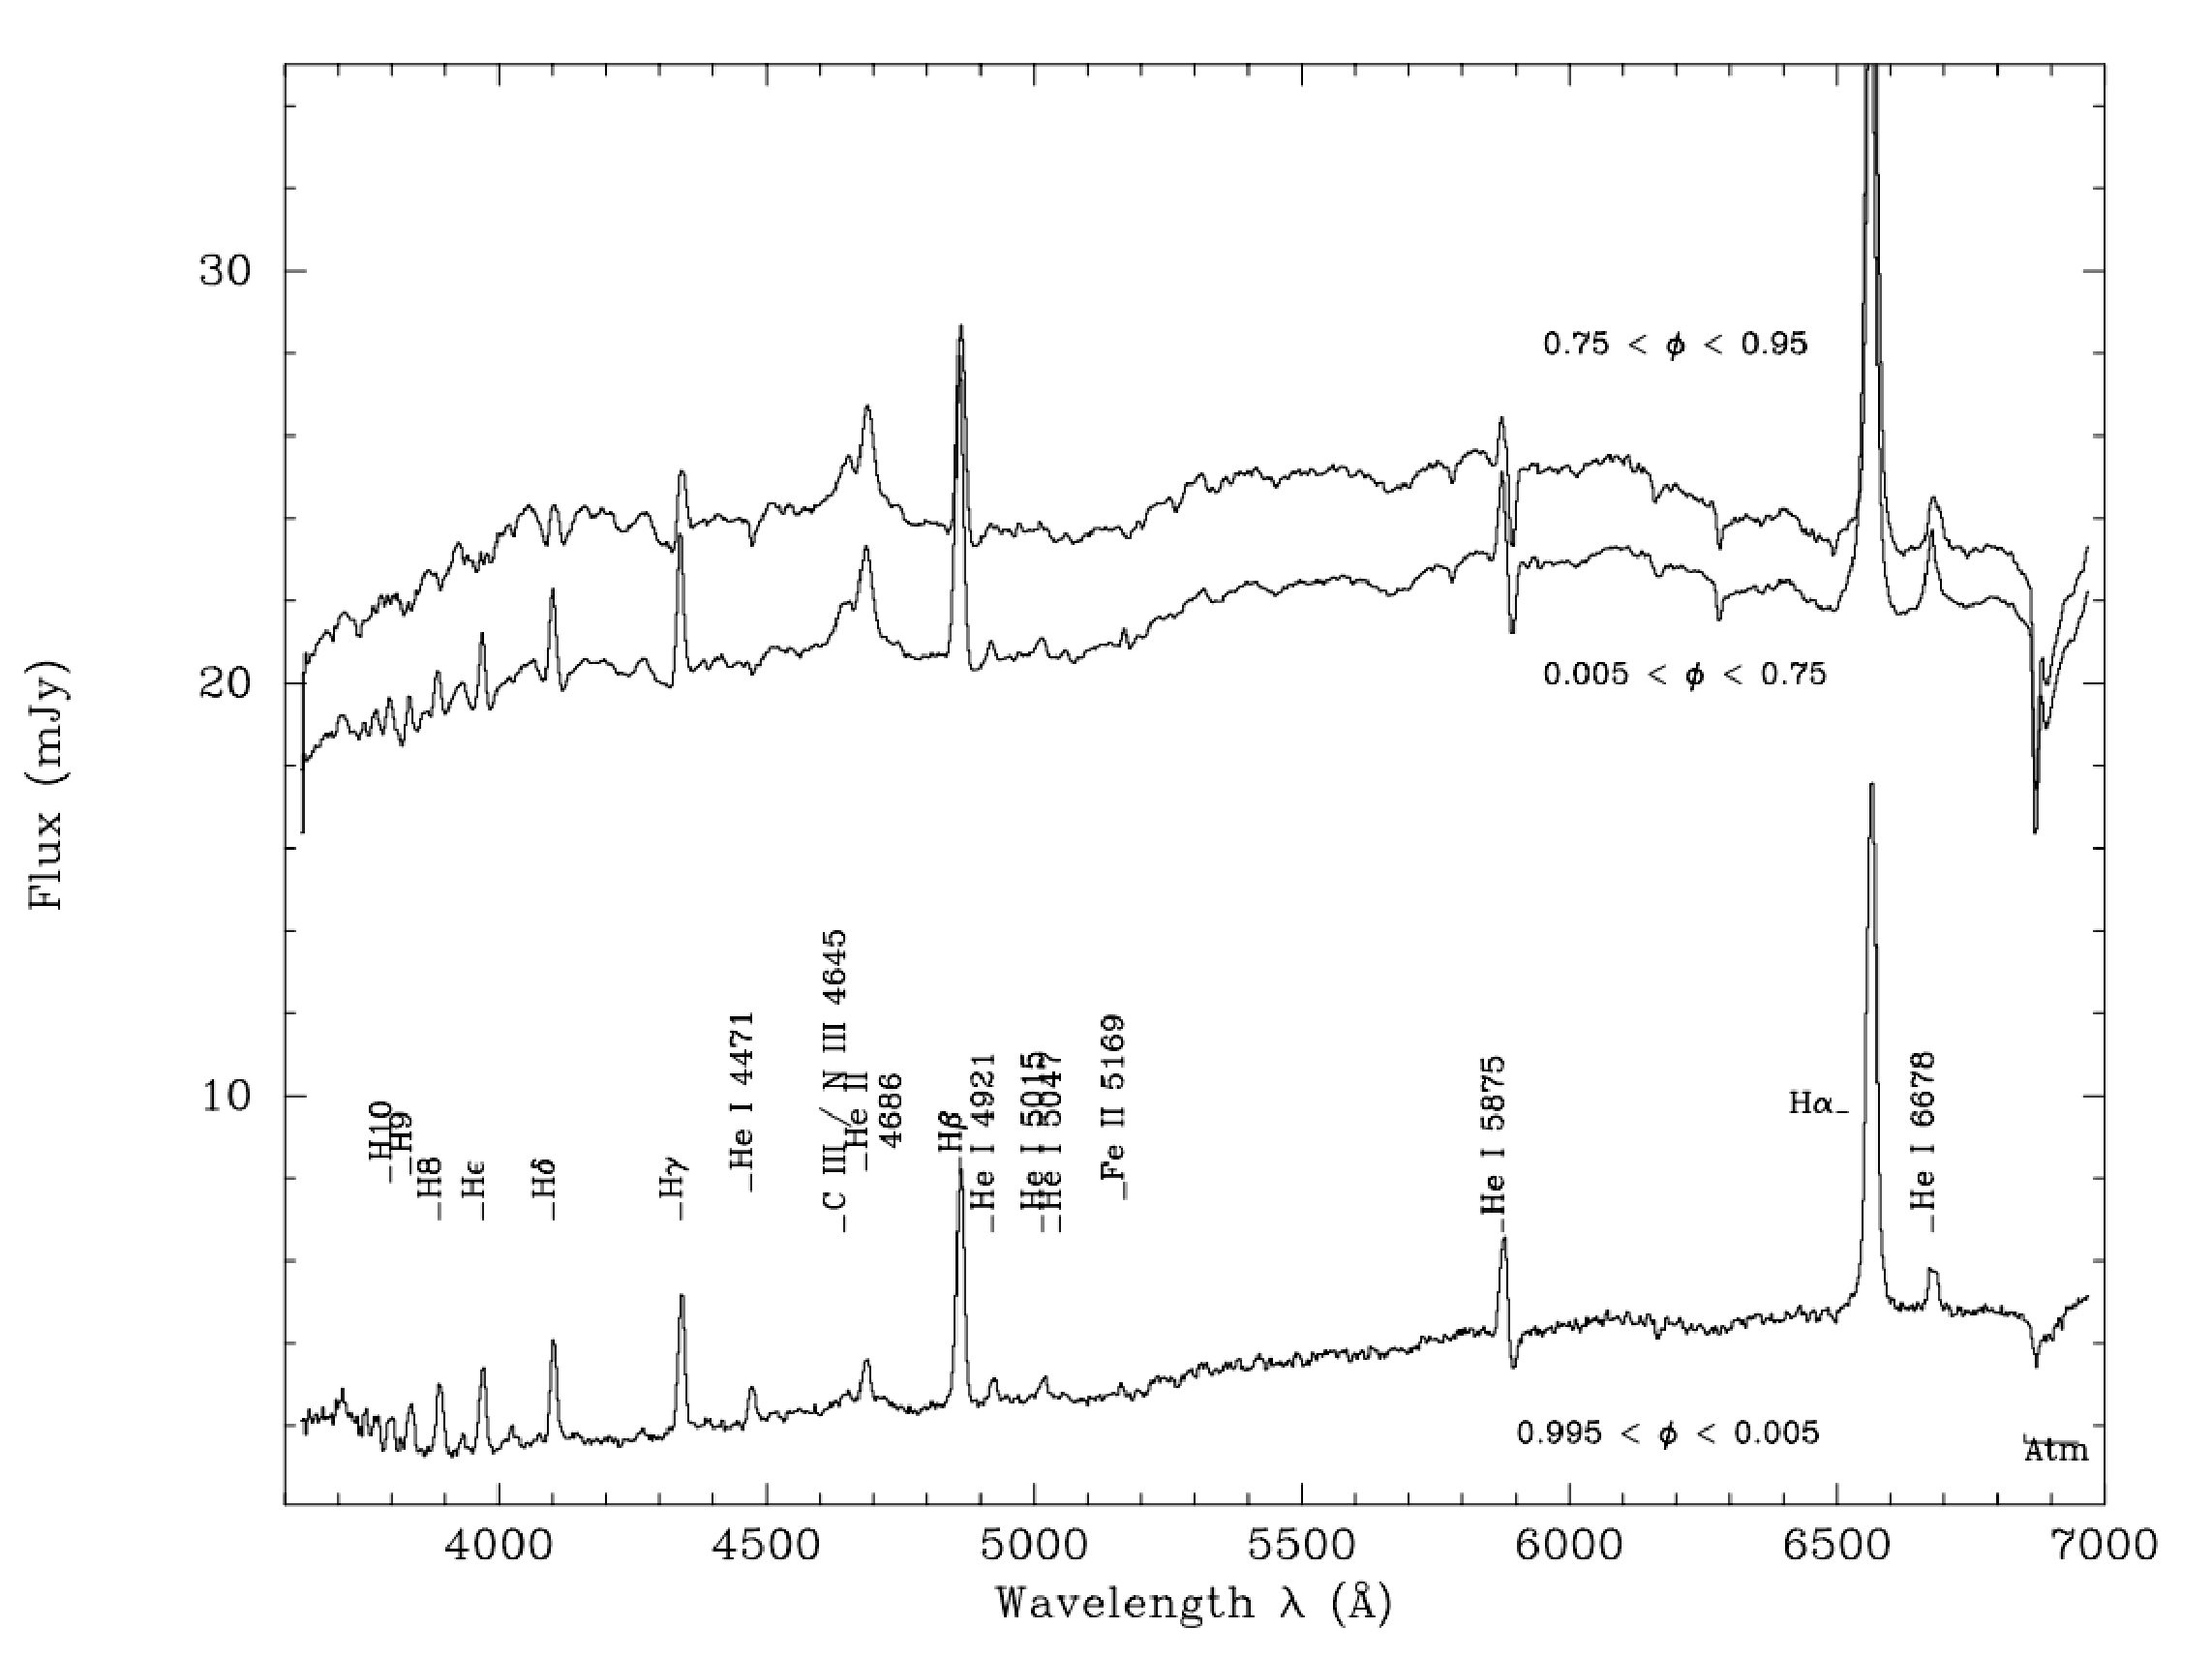
\includegraphics[width=1.0\textwidth]{figures/groot11.eps}
\caption{Optical Spectra of the high inclination Nova-like variable RW Triangulis.
Single peaked lines can be seen even in eclipse, suggesting that a wind may be responsible for 
the emission in these lines (figure from Groot et al. 2004).}
\label{spec}
\end{figure}


\begin{figure}[h]
\centering
\includegraphics[width=1.0\textwidth]{figures/plot_combined1.eps}
\caption{Optical ({\sl top}) and UV ({\sl bottom}) spectra from a Cataclysmic Variable model 
calculated with \py for three viewing angles corresponding 
to inclinations of 30 (blue), 60 (green) and 70 (red) degrees.
The transition from a P-Cygni like line profile to broad emission line in C\textsc{iv}  can be clearly seen, and there is also a noticeable dependence on inclination in the shape of the Balmer jump.}
\label{spec}
\end{figure}

% \begin{figure}[H]
% \centering
% \includegraphics[width=0.68\textwidth,clip=true, trim=0.2in 0in 0.2in 0.5in]{plot_combined1.eps} 
% \caption{
% Optical ({\sl top}) and UV ({\sl bottom}) spectra calculated with PYTHON for three viewing angles corresponding 
% to the inclinations of RW Sex, IX Vel and RW Tri respectively. 
% The transition from a P-Cygni like line profile to broad emission line in C\textsc{iv}  can be clearly seen, and there is also a noticeable dependence on inclination in the shape of the Balmer jump.
% }
% \end{figure}

% \begin{figure}[h]
% \centering
% 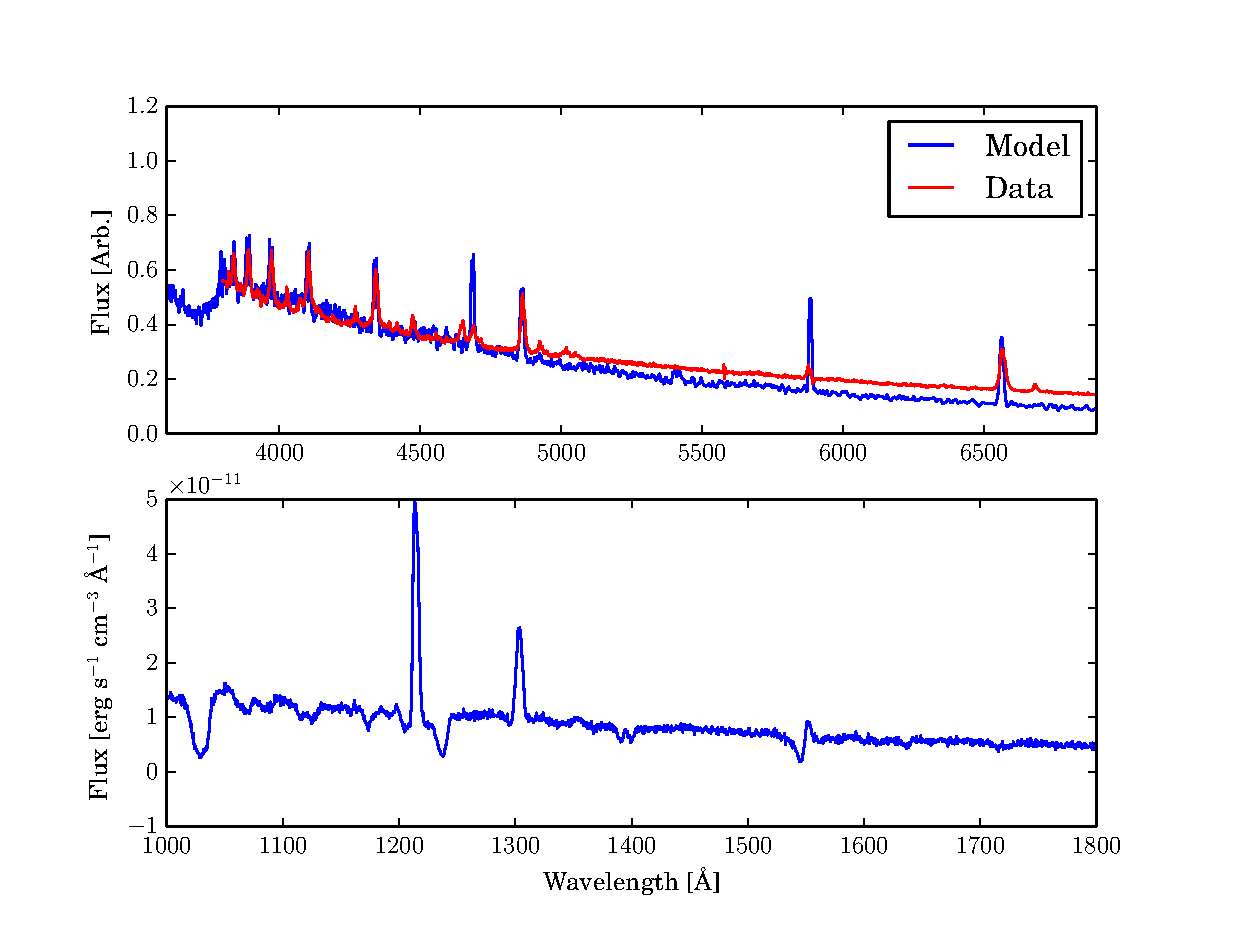
\includegraphics[width=0.5\textwidth]{figures/ixvel_sdss.eps}
% \caption{Cartoon illustrating the geomtry and kinematic properties of the wind.}
% \label{cartoon}
% \end{figure}

\subsection{Results}

{\bf Discussion of the spectra shown in Figure 3.}

\section{A Unified QSO Wind Model}

H13 present a benchmark disk wind model
which successfully reproduces some aspects of BALQSO spectra (see figure 5). However, inspection
of the model reveals three key shortcomings. First, the X-ray luminosity of the system
is weak. The unattenuated luminosity is already low for a BALQSO, and should be comparable
to a non-BAL QSO if a unified disk wind model is capable of explaining BALs. In addition,
X-rays are attenuated by the disk wind and mean that for BAL angles the luminosity observed
is low for a BALQSO. Second, the model fails to reproduce BELs, as not enough thermal line
emission is produced. Third, the fiducial model fails to correctly model the \la line, because
it uses the two-level atom approximation.
Fortunately, some progress has been made in addressing these three problems.

I have now improved the macro atom mode so that it can also deal
with compton processes using the framework implemented by Nick Higginbottom.
This simply involved adding an extra k-packet destruction channel for Compton 
heating, and k->r process for Compton cooling. 
It is now also possible to run the code in hybrid macro/simple-ion mode
using the improved ionization scheme presented by H13.
{\bf Here I will write something on QSO models I've run so far
with more line emission and include a relevant figure}.

\bigskip



%%%%%%%%%%%%%%%%%%%%%%%%%%%%%%%%%%%%%%
%
%          FUTURE WORK
%
%%%%%%%%%%%%%%%%%%%%%%%%%%%%%%%%%%%%%%%

\newpage
\section{Thesis Plan \& Summary}
\label{future}
\noindent Remaining work will be split between a number of projects, forming a thesis with a planned structure as follows.
\bigskip

\noindent {\bf Chapter 1: Introduction.} Context and relevant background.

\bigskip

\noindent {\bf Chapter 2: Accretion Disks and Their Winds.} A theoretical and observational overview of the evidence for accretion disk winds, and a review of our current understanding of disk and wind physics.

\bigskip

\noindent {\bf Chapter 3: Macro Atoms and Radiative Transfer.} A description of radiative transfer techniques used in \py and an outline of the macro-atom scheme and why it is so important.

\bigskip

\noindent {\bf Chapter 4: The Disk Wind Contribution to Optical Spectra of Cataclysmic Variables.} 

\noindent {\bf Timescale for completion:} 1-2 months (this project is in the writing up phase.)

\noindent {\bf Details:} Some results from this project are shown in Section 3. The broad conclusions are that when a full treatment of recombination is included then the emission from the wind is able to produce strong lines in Hydrogen and Helium, as well as providing 
sufficient continuum emission to mask the Balmer jump at some inclinations.

\bigskip

\noindent {\bf Chapter 5: A Disk Wind Unification Model for Quasi-Stellar Objects}

\noindent {\bf Timescale for completion:} 6-9 months

\noindent {\bf Details:} This project is a natural progression from previous work. Our team 
has already produced a proof-of-concept for the macro atom method in a CV context, and 
also presented a benchmark model for BALQSOs (H13). I will apply the macro atom method
to our benchmark QSO model, and coupled with a geometry parameter search this will provide insights
into whether or not a simple biconical wind geometry can produce Broad emission lines in 
resonance lines such as Carbon IV and lines such as Lyman-$\alpha$. This project
also provides the opportunity for collaboration with Francesco Shankhar who has identified
a way in which our code could be used in conjunction with his work
on the X-ray and optical properties of BALQSOs (see Morabito et al. 2013\nocite{morabito2013}).

\bigskip

\noindent {\bf Final Science Chapter (Potential): Disk Wind Modeling of X-ray Binaries}

\noindent {\bf Timescale for completion:} 6-9 months

\noindent {\bf Details:} P-Cygni line profiles in CIV have been observed in X-ray binaries,
offerring a tantalising hint of outflowing material \citep{ioannau2003}. I am a Co-I on the HST proposal 13630 which involves taking UV observations of the `missing-link' pulsar J1037, designed to assess the state of the wind when the system is in the accreting 
or radio pulsar stage of evolution. Modeling the system would provide an intriguing insight 
into the amount of mass loss and potential effects on the accretion disk, and would also
allow us to constrain the wind geometry. Even a wider-ranging, proof-of-concept investigation into
X-ray binary geometries would prove informative in both this context and more generally, using the groundwork
on X-ray systems in our code carried out by H13. This project offers the opportunity 
for collaboration with the Co-Is on proposal 13630: Diego Altamarino, Rene Breton
and Juan Hernandez Santisteban.

\bigskip

\noindent {\bf Final Science Chapter (Potential): Reverberation Modeling of Active Galactic Nuclei.}

\noindent {\bf Timescale for completion:} 6 months

\noindent {\bf Details:} Reverberation mapping is an important technique in understanding 
the geometry of AGN systems \citep{peterson1998}. Incorporating predictions for reverberation mapping
into our code is relatively straightforward; one simply has to track each individual 
photon's path length and origin as they travel through the wind. Once this is carried out,
predictions for reverberation responses can be made for various wind geometries, and a direct comparison
to reverberation mapping results will yield informative results and provide a well-defined project.

\bigskip

\noindent {\bf Chapter 7: Conclusions.} A summary of the work carried out and its implications for the field.

\bigskip
\noindent {\sl At a bare minimum}, I believe projects 1 \& 2 would provide sufficient 
original research to constitute a thesis, providing that project 2 involved significant development
of the benchmark H13 model and produced the anticipated high-impact work. 
However, given the time available, it is feasible that {\sl at least} one of the remaining projects 
will be completed in time for the final thesis. The choice of project undertaken will depend on a number of factors:

\begin{itemize}
 	\item The conclusions we can draw from the data from HST proposal 13630, and the implications for 
 	      modeling of X-ray binary winds
 	\item The ability of our model to produce BELs, as this impacts whether including reverberation mapping is
 	      possible, and indeed relevant.
 	\item The success of project 2 and the number of separate papers that come out of the study. 
 \end{itemize} 

 I believe a combination of the above projects presents a robust thesis plan.
The Phd will involve the application of Monte Carlo techniques to a number of different types of system, 
with the theme of unification and universality providing a scientific link between projects which 
 cover systems with masses ranging from one, to billions, of solar masses.





\section*{Acknowledgements}
I would like to thank the \textsc{Python} team for their invaluable help and for use of the code: Knox Long, Christian Knigge, Nick Higginbottom and Stuart Sim. In addition I would like to thank Christian Knigge for supervising this work. This document was prepared using the \texttt{mn2e} \textsc{Latex} macros, and simulation outputs are from \py 76. This work is supported by the Science and Technology Facilities Council (STFC).
%% \texttt{mn2e.cls} \textsc{Latex} document class. 


\bibliography{mybib.bib}
\newpage
%\appendix
\end{document}
